% This must be in the first 5 lines to tell arXiv to use pdfLaTeX, which is strongly recommended.
\pdfoutput=1
% In particular, the hyperref package requires pdfLaTeX in order to break URLs across lines.

\documentclass[11pt]{article}

% Change "review" to "final" to generate the final (sometimes called camera-ready) version.
% Change to "preprint" to generate a non-anonymous version with page numbers.
% \usepackage[review]{acl}
\usepackage[final]{acl}

% Standard package includes
\usepackage{times}
\usepackage{latexsym}
\usepackage{amsmath}
\usepackage{booktabs}
\usepackage{subcaption}
% \usepackage{hyp}

\newcommand{\model}{VisionSAM}

% For proper rendering and hyphenation of words containing Latin characters (including in bib files)
\usepackage[T1]{fontenc}
% For Vietnamese characters
% \usepackage[T5]{fontenc}
% See https://www.latex-project.org/help/documentation/encguide.pdf for other character sets

% This assumes your files are encoded as UTF8
\usepackage[utf8]{inputenc}

% This is not strictly necessary, and may be commented out,
% but it will improve the layout of the manuscript,
% and will typically save some space.
\usepackage{microtype}

% This is also not strictly necessary, and may be commented out.
% However, it will improve the aesthetics of text in
% the typewriter font.
\usepackage{inconsolata}

% If the title and author information does not fit in the area allocated, uncomment the following
%
%\setlength\titlebox{<dim>}
%
% and set <dim> to something 5cm or larger.


\usepackage{fancyhdr}

\usepackage{hyperref}

\usepackage{enumitem}

\usepackage{todonotes}

\title{Towards Smarter Segmentation: Improving SAM’s Anomaly Understanding with RLHF}

\author{
  Wan Wang \\
  University of Minnesota \\
  \texttt{wang9814@umn.edu}
  \And
  Yu-Tong Chuang \\
  University of Minnesota \\
  \texttt{chuan120@umn.edu}
  \And
  Lulin Liu \\
  University of Minnesota \\
  \texttt{liu02721@umn.edu}
  \And
  Yiu Chang \\
  University of Minnesota \\
  \texttt{chan2586@umn.edu}
}


\begin{document}

% Specify the document name here
\pagestyle{fancy}
%... then configure it.
\fancyhead{} % clear all header fields
\fancyhead[R]{\small{CSCI 5541 NLP S24}}
\fancyhead[L]{\small{Final Project}}
\fancyfoot{} % clear all footer fields
\fancyfoot[R]{\small\thepage}
% Some content:


\maketitle
\begin{abstract}
% balabala
% 老师上次的feedback
% 1. 报告格式改进: 要加摘要(abstract):未来提交的报告需要包含一个摘要,作为对整篇内容的简要概述。
% 2, 加强引用和论据支撑: 当你提到 “缺乏对异常的显式理解” 这种结论时,一定要加上参考文献或来源支持,不能只是主观判断。类似地,对于 “SAM在异常检测中存在困难” 的陈述,也要提供文献引用来支撑。
% 3, 澄清术语 / 模型细节: 关于你提到的“Rich Human Feedback”:这个反馈具体指的是什么?是不是意味着有人类偏好数据,还包含偏好理由?如果是,就要在报告中明确说明并解释清楚。
% 4, 选择合适的数据集 + 异常领域知识: 老师指出目前你们对数据集中的异常类型不太熟悉,这可能会影响你们的分析质量。
% 注意写Abstract,intro,说contribution的时候要注意措辞,用谦虚的态度。注意引用不要学术抄袭。
Industrial anomaly segmentation poses unique challenges due to the subtle, low-contrast nature of defects and the scarcity of high-quality annotations. While foundation models like Segment Anything Model (SAM) offer strong generalization in object-centric segmentation, they often fail to localize fine-grained anomalies. In this work, we make an initial attempt to adapt SAM to this setting via a two-stage pipeline: supervised fine-tuning (SFT) on a curated demonstration set, followed by preference-based finetuning using reinforcement learning from human feedback (RLHF). To facilitate this, we construct a small-scale comparison dataset with human-annotated segmentation preferences. Our method, VisionSAM, demonstrates modest yet consistent gains over the SFT baseline, achieving a +0.43\% IoU and +0.69\% Dice improvement on held-out categories. In contrast, directly applying RLHF to the original SAM results in performance degradation, underscoring the importance of task-specific grounding. Compared to existing fine-tuning strategies such as adapter-based or CLIP-integrated approaches, our method is the first to systematically introduce RLHF into dense prediction tasks. While results vary across prompt types and anomaly categories, our findings suggest that human-aligned feedback offers a promising supervision signal in low-data regimes, and opens a novel direction for human-in-the-loop vision foundation model adaptation.\footnote{Our code is available at \url{https://github.com/slmowan/sam-finetune}} \footnote{Please contact wang9814@umn.edu for the access permission if code check is needed.}
\end{abstract}


\section{Introduction}
% ------ Problem Definition -------
% 逻辑:
% 为什么工业界需要基于异常的视觉检测算法?业界需要solid的基于异常的视觉检测算法 --> 目的:替代人工质检, 自动化。
% 高质量数据 -> 更可靠的算法

% What problem do you try to solve? Describe your objectives cleraly without using any technical jargon. 
% 工业界需要robust,可解释的,solid的异常检测算法以最大程度的替代人工质检, 实现自动化流程。然而,现实的困境在于业界缺乏高质量异常分割数据以实现这类算法的supervised learning procedure, depends on access to high-quality segmentation data, which is often limited due to severe class imbalance in defect datasets and the high cost of pixel-level annotations requiring domain expertise. These constraints make large-scale supervised training impractical.
\textbf{Problem Definition.} In industrial settings, there is a growing demand for robust and interpretable anomaly detection algorithms to reduce reliance on manual inspection and enable end-to-end automation. However, a major challenge lies in the limited availability of high-quality segmentation data required for supervised learning. Industrial anomaly datasets typically suffer from severe class imbalance, where defective samples are rare, and collecting pixel-level annotations is both costly and time-consuming, often requiring domain-specific expertise. These limitations may hinder the advancement of supervised anomaly segmentation methods, especially in cases where model performance relies on access to large and diverse annotated datasets.

% ---------- Objective ----------
% There are two perspectives 来优化工业缺陷检测:1)model-centric perspective: 假设已经有了一定的数据质量(不去改变数据),重点是设计更好的模型结构、训练方法、后处理策略来提升性能; 2) data-centric perspective, which is focus on the quality of the data. 我们的项目更focus on 后者。如果能用更小的成本获得更优质的数据,就能有效提升模型表现,同时减少训练和迭代的资源浪费。因此,我们想尝试探索RLHF是否能够将异常知识注入vision foundation model that has the ability to segment从而能够帮助我们更轻易的制造更多的高质量数据。
% 数据质量 → 模型质量 的思路:如果能用更小的成本获得更优质的数据,就能有效提升模型表现,同时减少训练和迭代的资源浪费。
% objective相对于goal来说是更长期的目标,所以可以写的更大一些。
\textbf{Objective.} There are two perspectives for optimizing industrial defect detection. The model-centric perspective assumes a baseline level of data quality and focuses on improving model architectures, training strategies, or post-processing techniques to enhance performance. The data-centric perspective, on the other hand, emphasizes improving the quality and utility of the data itself. Our project focuses on the latter. We believe that obtaining higher-quality data at a lower cost can significantly improve model performance while reducing the resources required for training and iteration. To this end, we explore whether reinforcement learning from human feedback (RLHF) can inject anomaly-relevant knowledge into a vision foundation model with strong segmentation capabilities. Such a model could assist in generating more reliable pseudo-labels and facilitate scalable, data-efficient workflows for industrial inspection.

% ---------- Ohther researchers, Curent Gap ----------
% 现有的针对异常分割的方法中没有通过RLHF方法来改进LLM的尝试,我们想要弥补这个gap (这个地方逻辑不对)
% 没有提this gap是什么?
% To address this gap, we propose a novel approach: enhancing SAM with RLHF to integrate expert knowledge directly into its segmentation process. This work explores the feasibility of using RLHF to improve SAM’s performance in industrial anomaly segmentation, aiming to reduce dependency on costly manual annotations and to align segmentation outputs with expert-level understanding. To our knowledge, this is the first application of RLHF to vision-language segmentation models. 
% To our knowledge, this is the first application of RLHF to vision-language segmentation models. While RLHF has shown success in language and generative models, its potential in vision tasks remains underexplored. Our study bridges this gap and introduces a new paradigm for leveraging preference-based feedback to fine-tune segmentation models for domain-specific tasks. (novelty)
\textbf{Current Gap.} Existing approaches to adapting SAM for anomaly detection primarily focus on task-specific fine-tuning strategies. Notably, adapter-based methods such as HQ-SAM inject domain knowledge via lightweight modules, enabling improved performance on subtle industrial defects without retraining the entire model. Other efforts, like SAM-CLIP, incorporate knowledge distillation from multi-modal models (e.g., CLIP) to enhance segmentation by leveraging semantic cues through text-image alignment. While these methods have shown promising results, they still face key limitations: (1) they rely heavily on static supervision and lack mechanisms to incorporate dynamic, human-informed feedback; (2) they often struggle with precisely delineating low-contrast or ambiguous anomalies; and (3) they do not fundamentally address the model’s lack of an explicit “understanding” of what constitutes an anomaly. To date, no prior work has explored the use of human preference signals—such as those enabled by reinforcement learning from human feedback (RLHF)—to guide and refine SAM’s behavior in anomaly segmentation tasks, leaving a promising direction underexplored.


% ------ significance -------
% what is relevant stakehodlers?
\textbf{Significance.} This work is relevant to both industry practitioners and AI researchers. In industrial settings, current anomaly detection systems often rely on fully supervised training with dense pixel-level annotations, which are costly, time-consuming, and difficult to scale due to the rarity and subtlety of many defects. Vision Foundation Models such as SAM offer general segmentation capabilities but lack sensitivity to domain-specific anomalies, often under-performing on low-contrast or fine-grained defects. For researchers, this study offers a data-efficient alternative to traditional annotation-heavy methods. By introducing a human-guided adaptation framework, this work enables more practical fine-tuning of foundation models and has the potential to improve quality control, reduce waste, and enhance automation efficiency in industrial environments.  

% ------ impact -------
\textbf{Impact.} The main contributions of this report are summarized below:
\begin{enumerate}
    \item We make an initial attempt to explore the use of RLHF for industrial anomaly segmentation, illustrating its potential to enhance the adaptation of vision foundation models in domains where traditional supervision is limited.
    \item As a first attempt, we construct a small-scale, expert-annotated anomaly segmentation dataset to begin addressing the lack of high-quality industrial data and to facilitate exploration of human-in-the-loop learning under limited supervision. The dataset can be accessed \href{https://drive.google.com/file/d/1WrBl5hhJW4DL3Nobjv-YttYkrtiWpPJd/view?usp=sharing}{here}.
\end{enumerate}

    
\section{Related Work}
\textbf{Vision Foundation Models.} In recent years, VFMs have revolutionized computer vision by leveraging large-scale datasets and transformer-based architectures, mirroring the paradigm shift seen in Natural Language Processing (NLP) with models like GPT and BERT. Just as large language models (LLMs) have moved beyond task-specific training to enable zero-shot and few-shot learning across diverse NLP tasks, VFMs are designed to be general-purpose models capable of adapting to a wide range of downstream vision tasks, including object detection, segmentation, and image understanding. Two prominent VFMs that have significantly influenced vision-language research are SAM \cite{kirillov2023segment} and Contrastive Language-Image Pretraining (CLIP) \cite{radford2021learningtransferablevisualmodels}

SAM, developed by Meta AI, is a foundation model for image segmentation with unprecedented zero-shot capability. Trained on over 11 million images and 1 billion masks, it enables segmentation via prompt-based inputs such as points, bounding boxes, or textual descriptions, similar to how LLMs generate text from prompts. SAM is chosen as the pre-trained model for this study due to its pixel-level segmentation capability, which is crucial for fine-grained anomaly detection.


\textbf{Current finetuning methods for Vision Language Models in anomaly detection.} Existing fine-tuning approaches for vision-language models can be broadly categorized into three methods: 1) Adapter-based fine-tuning, which injects domain-specific knowledge into large models but may not fully capture anomaly characteristics such as HQ-SAM\cite{ke2023segmenthighquality}. 2) Knowledge distillation, which integrates multiple models (e.g., combining SAM and CLIP into a unified vision transformer), yet balancing knowledge transfer remains a challenge such as SAM-CLIP\cite{wang2024samclipmergingvisionfoundation}. 3) Zero-shot methods, which leverage pre-trained features but often fail to precisely segment anomalies due to limited domain adaptation such as WinCLIP\cite{jeong2023winclipzerofewshotanomalyclassification}. Despite their effectiveness in some domains, these methods still struggle to align segmentation results with human intent, especially in anomaly detection scenarios where understanding subtle defects is critical. Empirical evidence suggests that even fine-tuned SAM models lack a deep understanding of what constitutes an anomaly and often fail to generate accurate segmentation masks.

\textbf{RLHF in T2I Generation}. RLHF enhances text-to-image (T2I) generation by aligning outputs with human preferences. While models like Stable Diffusion and DALL·E leverage large-scale datasets, they often produce misaligned results, such as low fidelity, unrealistic details, or incorrect compositions. RLHF refines generation through iterative learning from human feedback, improving coherence, aesthetics, and fine-grained control.
A work proposed by Liang et al.\cite{liang2024richhumanfeedbacktexttoimage} introduces Rich Human Feedback (RHF) for T2I generation, proposing a fine-grained preference learning framework that refines generative outputs beyond simple binary reward signals. Instead of traditional reinforcement learning based on sparse rewards, RHF incorporates structured human feedback, allowing the model to learn nuanced quality distinctions in generated images. The results demonstrate that RLHF significantly improves image realism, adherence to textual descriptions, and user satisfaction.


\section{Method}

% What did you do exactly? How did you solve the problem? Why did you , think it would be successful? What is your hypothesis?

% What challenges did you anticipate and/or encounter during the , development of your approach? Did the very first thing you tried work? 这个challenge就写PPO的难点。

% What is scientific novel of your approach to address the , challenges?

% 写phase1, phase2, phase3
% A series of experiments on the SAM will be conducted to identify its limitations in the target domain, providing an insight into its segmentation weaknesses. Inspired by MedSAM \cite{wu2023medicalsamadapteradapting}, a domain-specific SAM model will be trained to serve as a baseline for comparison. Then, RLHF-based fine-tuning will be applied to the pre-trained SAM model to assess whether human-in-the-loop reinforcement learning can enhance segmentation quality. 


% workflow图挪到中间,放大, 最好用矢量图, Caption需要修改一下。
% 2025/5/7: 这个workflow需要引用一下相关的work. (bib还需要补充文献)
\begin{figure*}[tb]
    \centering
    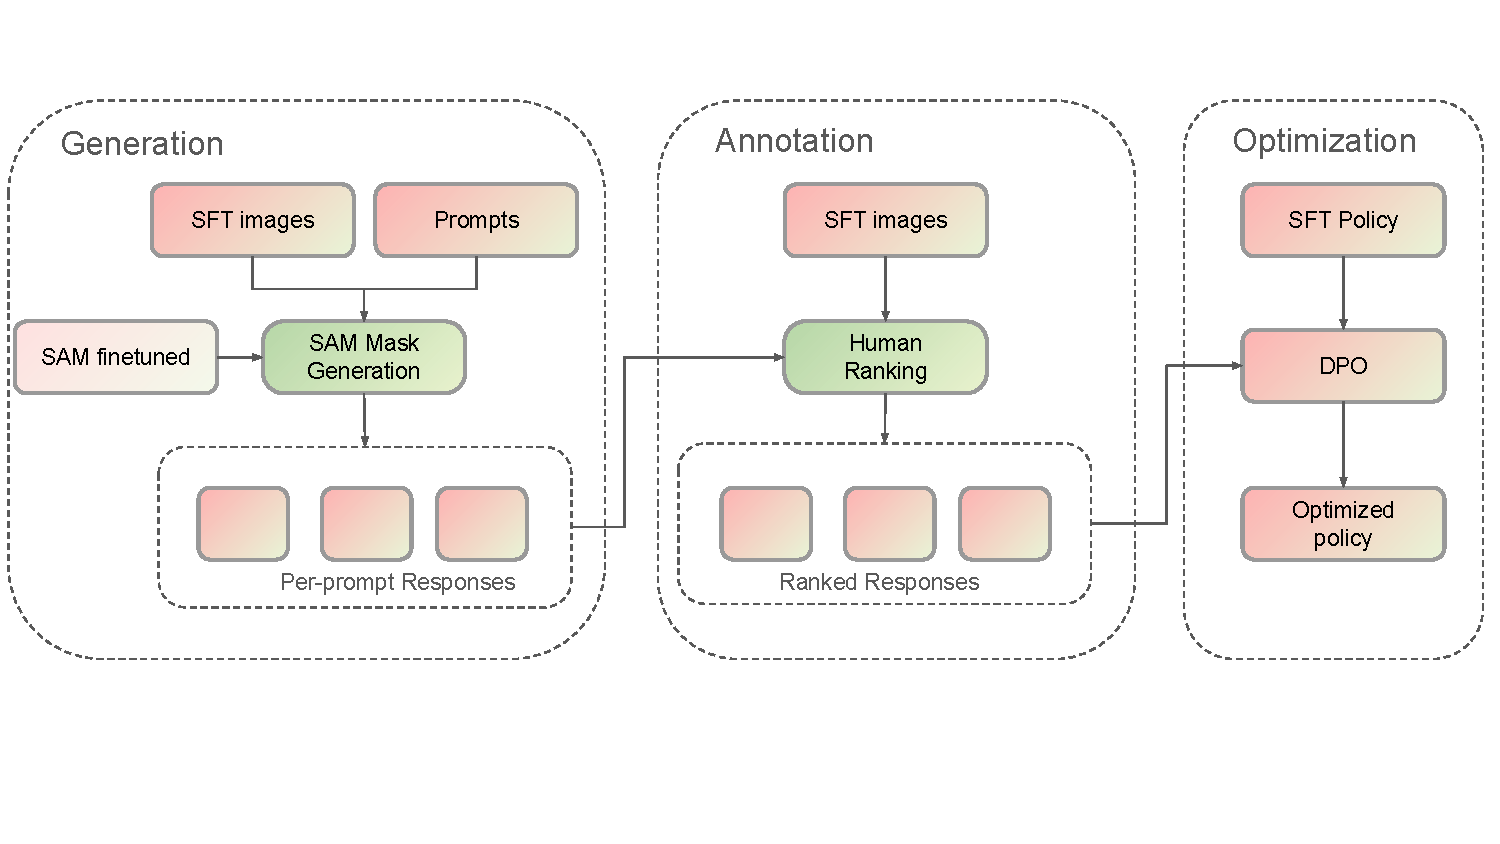
\includegraphics[width=0.8\textwidth]{figs/pipeline.pdf}
    \caption{Overview of our RLHF-based fine-tuning workflow for segmentation. The pipeline consists of three stages: (1) Generation — SAM generates multiple masks per prompt; (2) Annotation — humans rank the masks based on quality; (3) Optimization — preference data is used to fine-tune the model via Direct Preference Optimization (DPO).}
    \label{fig:training_pipeline}
\end{figure*}


\subsection{Datasets}
% 关于VISION数据集
% 关键词:工业、异常
% 14个异常类别: Cable, Capacitor, Casting, Console, Cylinder, Electronics, Groove, Hemisphere, Lens, PCB_1, PCB_2, Ring, Screw, Wood.
% 44个defect types
% 可以放一个数据的visualization
% 这个数据集有什么特点?
% 数据集的总数据量有多少?
We mainly utilize the \href{https://huggingface.co/datasets/VISION-Workshop/VISION-Datasets}{VISION dataset} for our project, which is a comprehensive and realistic benchmark specifically designed for industrial anomaly detection and segmentation. It includes 14 representative inspection categories (e.g., Cable, Capacitor), with approximately 18,000 high-resolution images captured across diverse manufacturing settings. The dataset's anomalies are often subtle, low-contrast, and embedded in complex visual contexts, making it a challenging and representative setting for evaluating the effectiveness of our proposed methods.

We also used \href{https://www.mvtec.com/company/research/datasets/mvtec-ad}{MVTec AD} dataset in our phase 1 analysis.

% \subsection{Problem Definition}
% % Enhancing the Segmentation Performance of SAM Using RLHF in Vision-Language Models
% Despite its strong zero-shot segmentation ability, SAM struggles with anomaly detection, lacking an explicit understanding of domain-specific defects. Existing fine-tuning methods attempt to adapt SAM but still face challenges in capturing the nuanced nature of anomalies. This highlights the need for a new fine-tuning approach that integrates human expertise without relying on extensive manual annotations.

%How did you solve the problem?
% We aim to develop an automatic annotation tools as well as investigate the potential of RLHF in improving SAM’s anomaly segmentation capability. If RLHF proves effective, it could provide a scalable, human-aligned fine-tuning strategy that improves segmentation accuracy and reduces the need for costly annotations. This study's objective is to bridge this gap by implementing and evaluating RLHF-based fine-tuning for SAM, assessing its impact on segmentation quality, domain adaptation, and practical deployment in anomaly detection tasks.

\subsection{Motivating Fine-Tuning: Where SAM Falls Short}
% 在这个阶段提出假设, 回答这个问题:Why did you think it would be successful? What is your hypothesis?
Prior to the generation stage of the RLHF-Based Segmentation Fine-Tuning Workflow, we first evaluate SAM’s segmentation performance on the \href{https://www.mvtec.com/company/research/datasets/mvtec-ad}{MVTec AD} dataset to analyze its failure modes anMehd performance boundaries under diverse industrial anomaly scenarios. Specifically, we uniformly sample 210 test images from 14 distinct anomaly categories (e.g., Cable, Pill, Bottle, Metal Nut), with 10 to 15 representative instances per category. This sampling strategy ensures broad coverage across variations in defect shape, texture, and scale, providing a solid foundation for assessing SAM’s zero-shot generalization capability.

Preliminary Results (will disclose in next section) show that despite its strong zero-shot segmentation ability, SAM struggles with anomaly detection, lacking an explicit understanding of domain-specific defects in some situations. Existing fine-tuning methods attempt to adapt SAM but still face challenges in capturing the nuanced nature of anomalies. This highlights the need for a new fine-tuning approach that integrates human expertise without relying on extensive manual annotations.

We hypothesize that human preference signals—particularly when leveraged through reinforcement learning from human feedback (RLHF)—can serve as an effective supervision alternative by guiding the model toward segmentation outcomes that align more closely with human judgment. Given SAM’s strong base segmentation capability, we believe that even limited preference-based feedback can steer the model to better capture subtle anomaly patterns that traditional supervision may overlook.

\subsection{RLHF-Based Segmentation Fine-Tuning Workflow}
% What did you do exactly? How did you solve the problem? Why did you , think it would be successful? What is your hypothesis?
We adopt a three-stage RLHF-based fine-tuning workflow inspired by InstructGPT framework~\cite{ouyang2022traininglanguagemodelsfollow}, with necessary adaptations for the segmentation task. While InstructGPT focuses on aligning language models with human preferences through reward modeling, our workflow extends this concept to the vision domain, aiming to align segmentation outputs with human perveptual judgments. As illustrated in Figure 1, the overall workflow consists of three sequential stages: (1) \textbf{Generation}, where a fine-tuned SAM model produces multiple segmentation masks in response to human-designed prompts; (2) \textbf{Annotation}, where human annotators rank these masks based on a rubric, creating preference-labeled data; and (3) \textbf{Optimization}, where we apply Direct Preference Optimization (DPO) to further align the model’s predictions with human preferences.

During the Generation stage, we first construct a supervised fine-tuning (SFT) dataset to initialize a domain-adapted SAM model. To ensure high signal quality for learning, we manually filtered approximately 500 images from the VISION dataset, selecting samples that (1) exhibit clearly visible anomalies and (2) have minimal background clutter. These images span multiple defect categories and were selected to balance shape, texture, and defect scale diversity. For each selected image, we use a sparse box prompt centered around the annotated defect region, simulating minimal human input. These prompt-image pairs (see \autoref{fig:sam_triplet}) are then fed into a lightly modified version of SAM (ViT-B variant), where we freeze the image encoder and fine-tune only the mask decoder layers. The model is trained using classical binary cross-entropy loss. During inference, we retain SAM’s native multi-mask decoding mechanism, generating three candidate masks per prompt to facilitate downstream human preference annotation.

% 这里可以放张图片展示一下sam_triplet sample
\begin{figure}[ht]
  \centering
  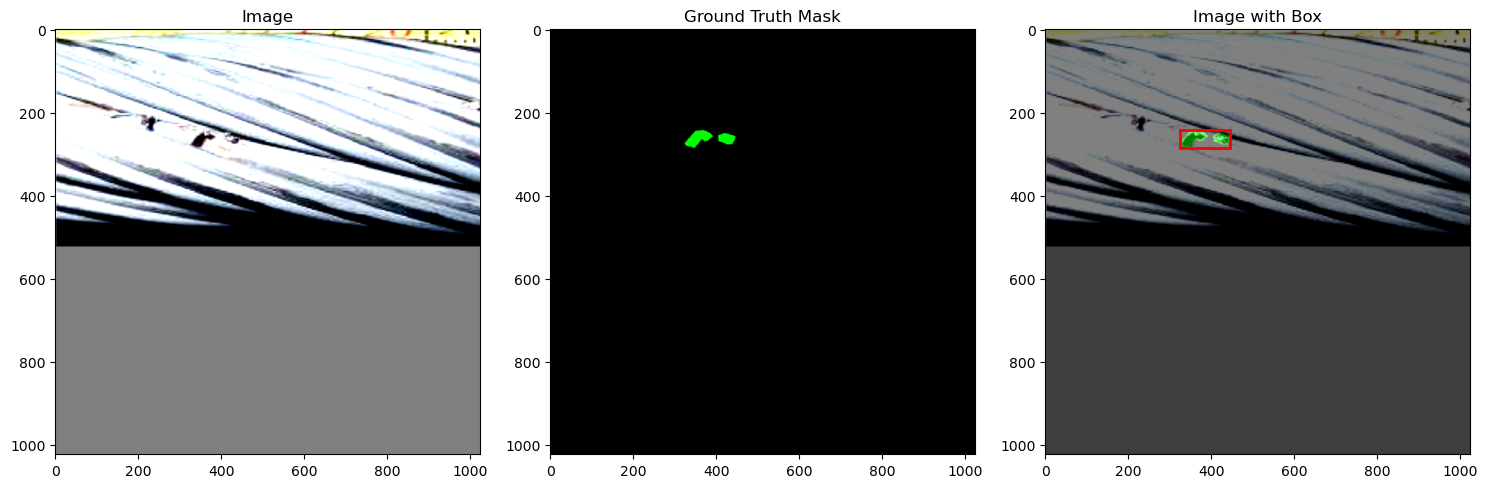
\includegraphics[width=1\linewidth]{figs/sam_triplet_sample.png}
  \caption{An example of a SAM-compatible triplet training sample.}
  \label{fig:sam_triplet}
\end{figure}


In the Annotation stage, we incorporate human-in-the-loop feedback to create high-quality preference data. All four authors participated in the annotation process. To ensure consistency, we first reviewed several anomaly segmentation benchmarks (e.g., MVTec AD, DAGM) and conducted a brief internal calibration session to align on quality criteria. Based on this, we collaboratively designed a rubric focusing on four key aspects: (1) coverage of the anomalous region, (2) boundary accuracy, (3) over-segmentation or under-segmentation, and (4) noise or spurious artifacts. For each prompt and image pair, the SAM-based model generates three candidate masks with varying internal confidence scores. Annotators independently examined these outputs and used the rubric to rank them. From each set, we selected the most preferred and least preferred masks, forming comparison triplets in the format: (prompt, preferred mask, rejected mask). These ranked responses serve as supervision signals in the preference-based fine-tuning stage.

% 需要描述一下如何利用annotation stage产生的comparison dataset进行训练的。1)训练模型时喂给模型的input是什么;2)模型如何使用DPO优化的过程;3)最后得到的output是什么--> 一个optimized policy。可以说一下这里的policy是什么(异常)。4)training时候用到什么超参数可以稍微提一提增加真实性。5)你认为training的时候有没有什么注意点,踩的坑之类的。
In the final optimization stage, the goal is to fine-tune the SAM model using the comparision dataset from the annotation stage. Each training instance consists of an input image, a bounding box prompt, and a pair of segmentation masks: a preferred mask (chosen) and a rejected mask. We frame this as a preference learning task and adopt Direct Preference Optimization (DPO) to align the model’s outputs with human feedback. During training, the model receives an RGB image resize to $1024 \times 1024$, a bounding box prompt in the format $[x1, y1, x2, y2]$, and the two corresponding masks, both converted to binary tensors and resized to $256 \times 256$ for stable loss computation. The SAM mask decoder processes the image and prompt to produce a predicted segmentation mask. This prediction is then compared against both the preferred and rejected masks using binary cross-entropy (BCE) to compute scalar reward scores $r_{\text{chosen}}$ and $r_{\text{rejected}}$, respectively.

These reward values are passed into the DPO loss function:

% We froze all vit\_b SAM components except the mask decoder and optimized using Adam optimizer with 1e-5 learning rate. (这句话和之前的稍微有些重复了) We passed each of the the image in the dataset trough the image encoder (frozen) and extracted the image embeddings. The bounding box prompt was also encoded with the prompt encoder.

% DPO的loss公式放在这里。可以描述一下training的时候如何utilize这个DPO的loss来optimize的。

\begin{equation}
\mathcal{L} = -\frac{1}{N} \sum_{i=1}^{N} \log \left( \sigma\left( \beta \left( r^{(i)}_{\text{chosen}} - r^{(i)}_{\text{rejected}} \right) \right) \right)
\end{equation}
where $\sigma(\cdot)$ denotes the sigmoid function and $\beta$ is a temperature hyperparameter (set to 1.0 in our experiments) that controls the sharpness of preference distinctions.

This formulation penalizes the model when its predictions align more closely with the rejected mask than with the preferred one, thereby encouraging the decoder to internalize human perceptual preferences. The output of this stage is an updated segmentation policy—represented by the fine-tuned decoder—that produces masks more consistent with our pseudo-expert judgments.

% novel proposed idea and your execution plan (noverlty: compare to the state of the art methods/systems/datasets, how novel is your approach?)

% Need to add illustration?
\section{Experiments and Results}
% RLHF finetune后模型的param size增加了, 为什么?

\subsection{Experimental setup}
% 这里放training loss图
\begin{figure}[ht]
  \centering
  \begin{subfigure}[t]{0.48\linewidth}
    \centering
    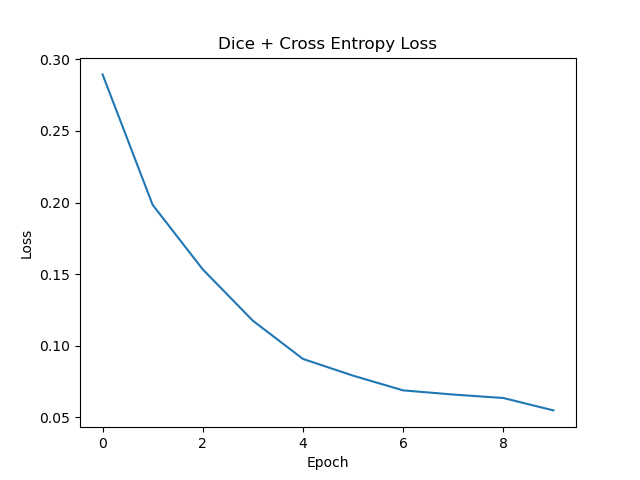
\includegraphics[width=\linewidth]{figs/sft_train.png}
    \caption{SFT-SAM training loss.}
    \label{fig:sft-loss}
  \end{subfigure}
  \hfill
  \begin{subfigure}[t]{0.48\linewidth}
    \centering
    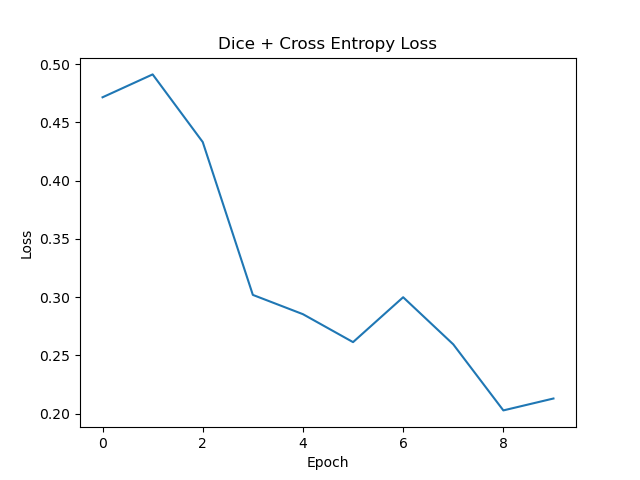
\includegraphics[width=\linewidth]{figs/dpo_train.png}
    \caption{VisionSAM training loss.}
    \label{fig:vision-loss}
  \end{subfigure}
  \caption{Training loss curves for models in two stages.}
  \label{fig:loss-comparison}
\end{figure}

Figure~\ref{fig:loss-comparison} presents the training loss curves for the SFT-only model (SFT-SAM) and the RLHF-enhanced model (VisionSAM). SFT-SAM is trained on our manually curated demonstration dataset, while VisionSAM is optimized using the comparison dataset derived from human preference annotations.

\textbf{Evaluation Metrics.} During inference, we evaluate model performance using two standard segmentation metrics: Intersection over Union (IoU) and Dice coefficient. These metrics are widely used in segmentation tasks for assessing the overlap between predicted and ground truth masks.

\textbf{Baselines.} We consider both the original SAM model and our fine-tuned SAM model as baselines for comparison. All models are evaluated under identical settings to ensure a fair assessment. Original SAM refers to the ViT-B variant for all experiments unless otherwise specified. While our current study focuses on ViT-B due to its favorable trade-off between performance and efficiency, future work may explore larger variants such as ViT-L and ViT-H to assess the effect of model scale on anomaly segmentation performance.


% Experiments with the same settting are conducted on several categories. 

\subsection{Results and Analysis}
\subsubsection{Baseline Behavior: SAM’s Response to Anomaly Prompts}

We adopt the original SAM as our baseline in this stage. To examine the impact of different prompting strategies on SAM’s segmentation quality, we tested three prompt configurations: 1) Single positive point: One point indicating the center of the target defect; 2) Positive + Negative point: A positive point on the target and a negative point in a distractor region; 3) Bounding box: A tight box enclosing the target anomaly.

\autoref{fig:sam_result} presents four representative results, covering a range of typical outcomes observed in our Phase 1 analysis: 

1) Correct Segmentation, Aligned Confidence: In some cases (e.g., Row 1), SAM successfully produces a mask that closely matches the ground truth in both shape and location. Additionally, the mask with the highest confidence score corresponds to the best segmentation, indicating a strong alignment between model prediction and human judgment. These are ideal cases where SAM functions as expected; 

2) Correct Segmentation, Misaligned Confidence: In cases like Row 2, SAM generates a reasonably accurate mask (e.g., Mask 2 with score = 0.512), but assigns a higher confidence to a suboptimal one (e.g., Mask 1 with score = 0.945). This discrepancy suggests a misalignment between the model’s internal scoring and human perception of quality. Such behavior might hinder downstream automation systems that rely on score-based mask selection.
    
3) Partial Failure due to Semantic Misunderstanding: In Row 3, SAM sometimes segments entire object structures rather than focusing on the anomalous regions. For example, when tasked with segmenting a defect on a wire, SAM includes the inner cavity of the wire as part of the predicted mask. While the mask is spatially consistent, it reflects a lack of semantic understanding of what constitutes a defect, highlighting SAM’s bias toward object-level rather than anomaly-level segmentation.
    
4) Failure Cases with Subtle Defects: Row 4 demonstrate cases where SAM fails to produce any meaningful segmentation. In Row 4, the anomaly (a slight deformation in a carpet) is barely perceptible even to human observers.

Across all experiments, we observed that SAM often segments entire objects rather than focusing on local defects, suggesting it lacks an explicit notion of “anomaly.” Point-based prompts, especially those combining positive and negative clicks, generally led to better results than bounding boxes, likely due to the finer spatial guidance they provide.

\begin{figure*}[t]
	\centering
        % 情况1: 分的好,且模型给出的分数和人是一致的
        % metal
	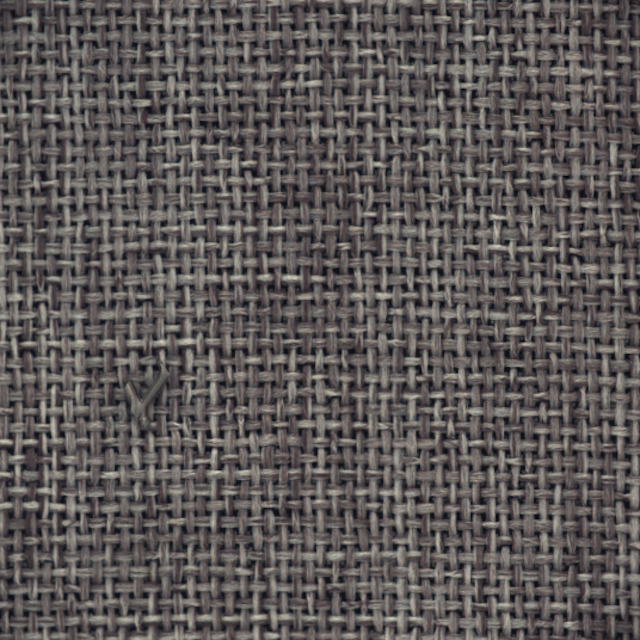
\includegraphics[width=0.19\linewidth]{figs/phase_1/metal_1.png}
        
\includegraphics[width=0.19\linewidth]{figs/phase_1/metal_2.png}
        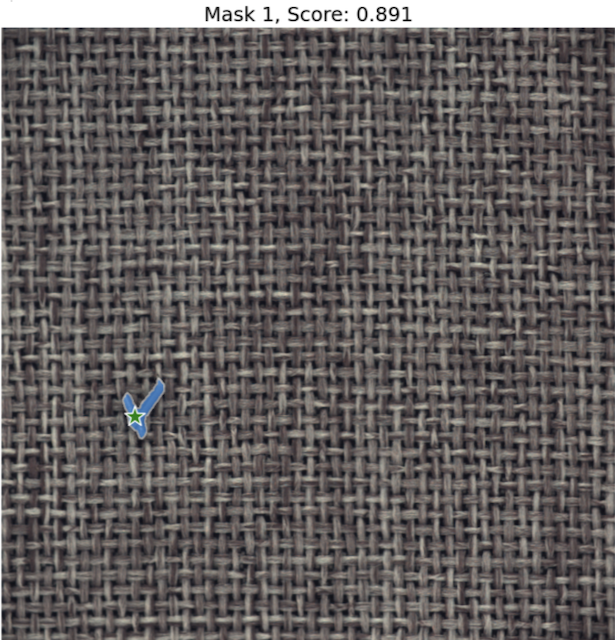
\includegraphics[width=0.19\linewidth]{figs/phase_1/metal_3.png}
        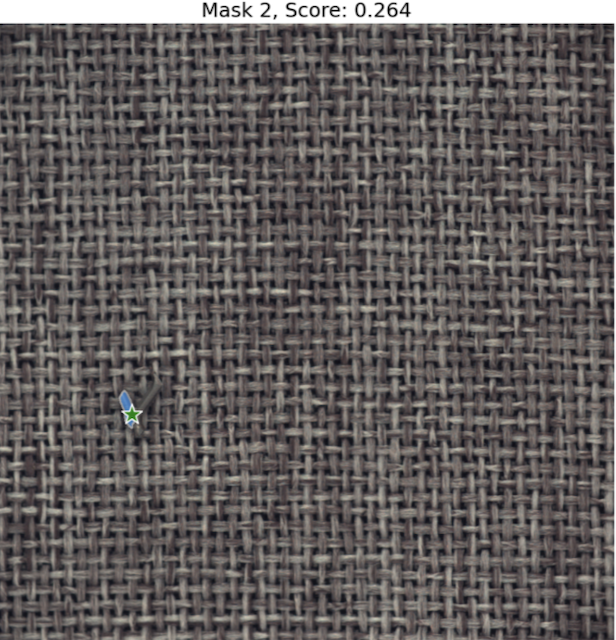
\includegraphics[width=0.19\linewidth]{figs/phase_1/metal_4.png}
        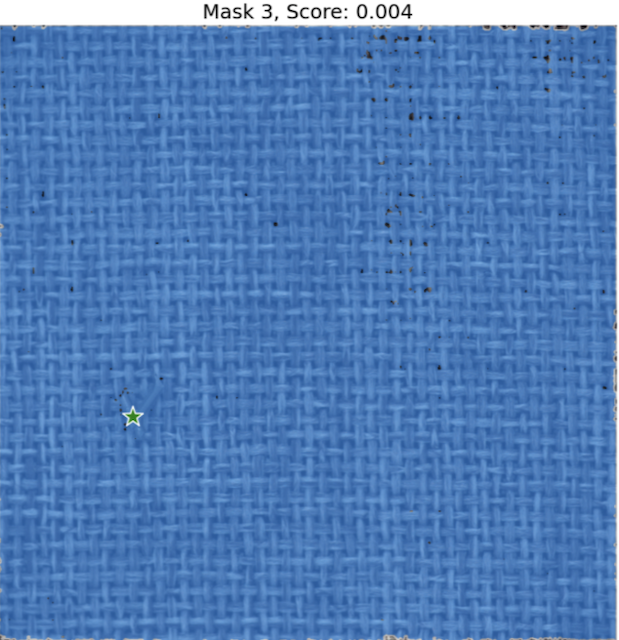
\includegraphics[width=0.19\linewidth]{figs/phase_1/metal_5.png}

        % 情况2: 分的好,但是模型给出的分数和人的分数不一致
        % crack
        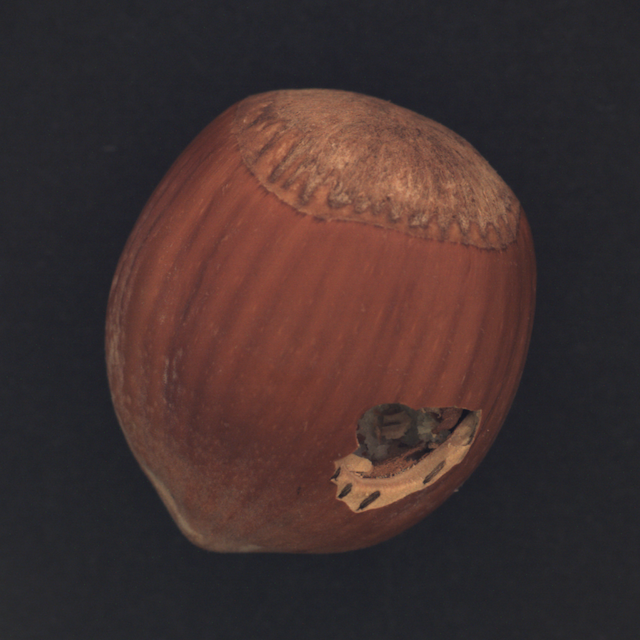
\includegraphics[width=0.19\linewidth]{figs/phase_1/crack_1.png}
        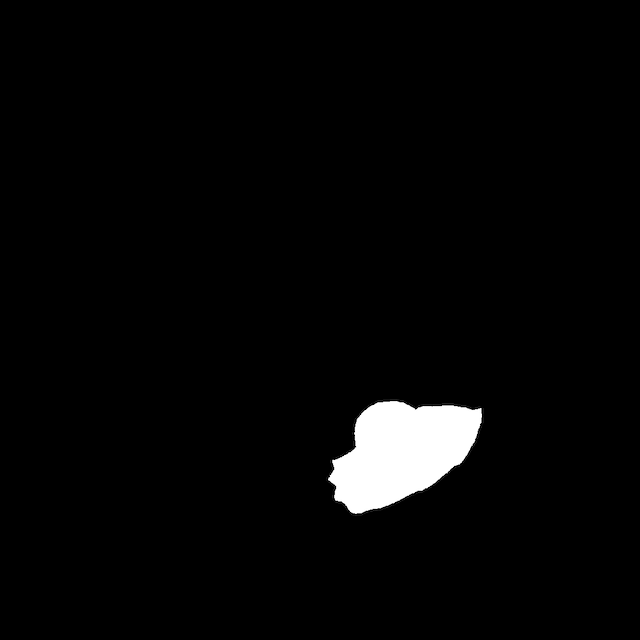
\includegraphics[width=0.19\linewidth]{figs/phase_1/crack_2.png}
        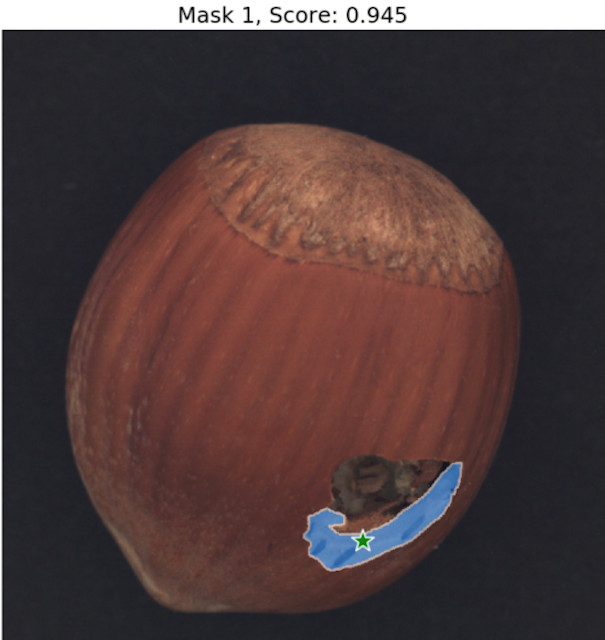
\includegraphics[width=0.19\linewidth]{figs/phase_1/crack_3.png}
        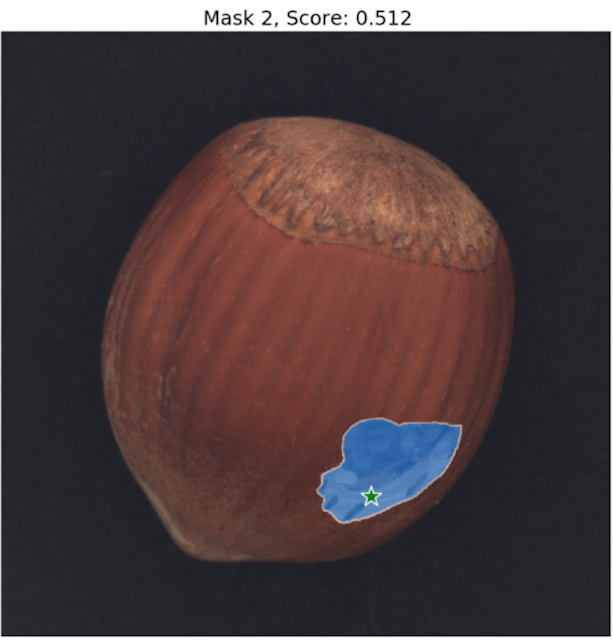
\includegraphics[width=0.19\linewidth]{figs/phase_1/crack_4.png}
        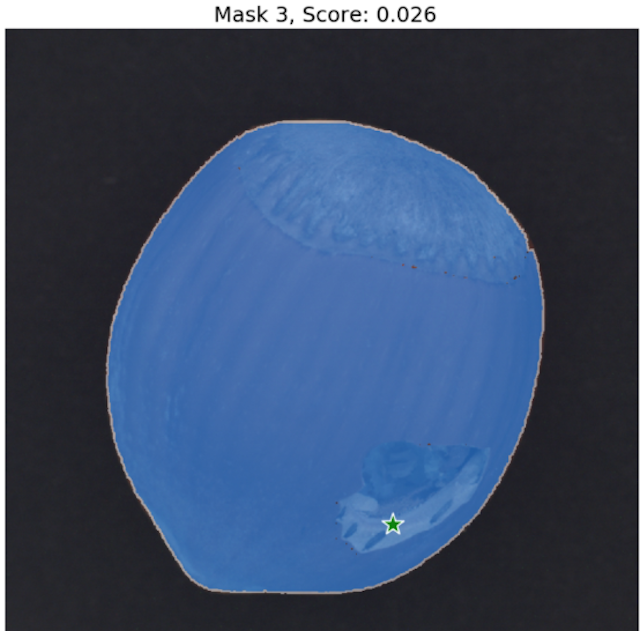
\includegraphics[width=0.19\linewidth]{figs/phase_1/crack_5.png}
	% \vspace{-.1in}

        % 情况3: failure cases (partial fail): 能够分出大致的结构,但是缺乏对异常的理解
        % missing wire
        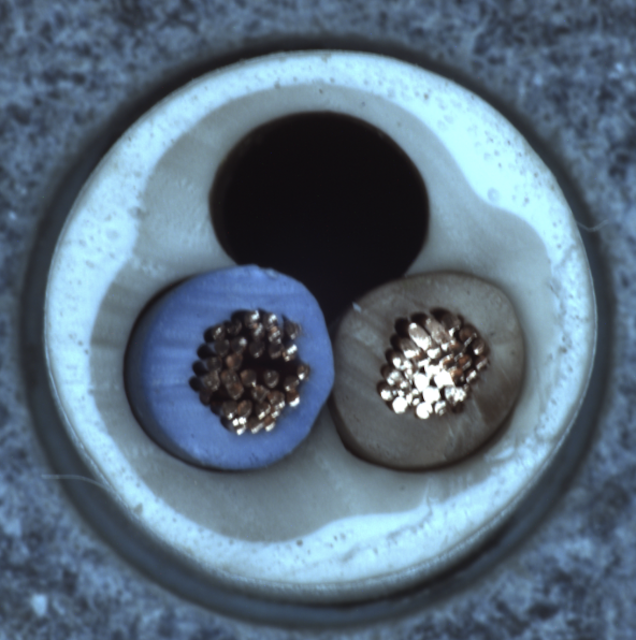
\includegraphics[width=0.19\linewidth]{figs/phase_1/missing_wire_1.png}
        
\includegraphics[width=0.19\linewidth]{figs/phase_1/missing_wire_2.png}
        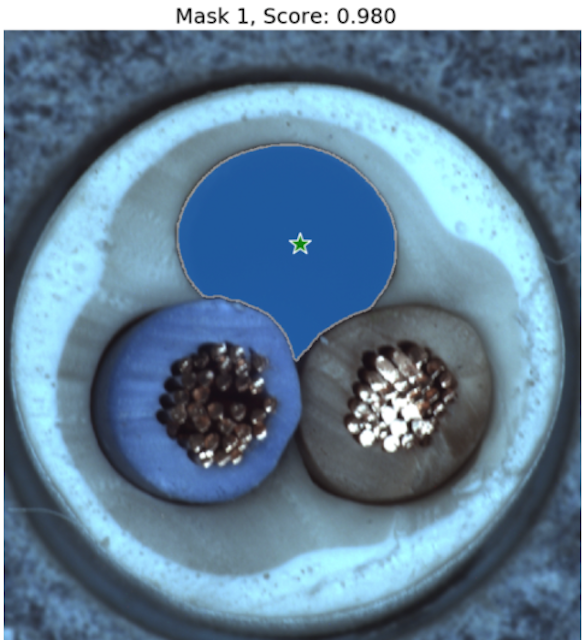
\includegraphics[width=0.19\linewidth]{figs/phase_1/missing_wire_3.png}
        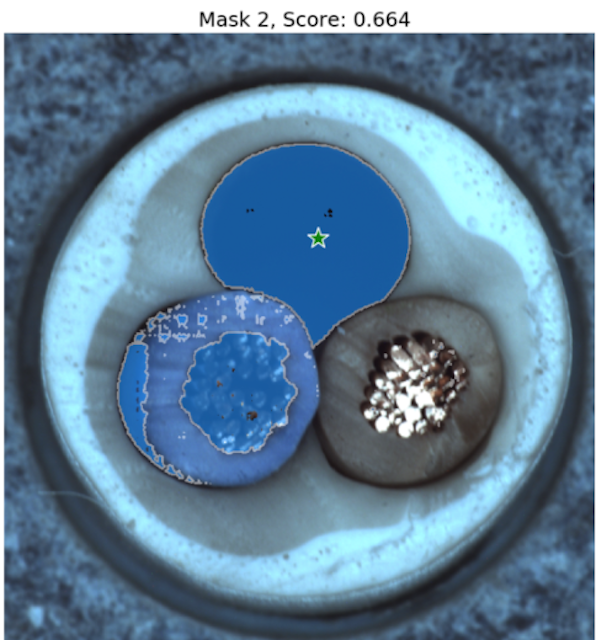
\includegraphics[width=0.19\linewidth]{figs/phase_1/missing_wire_4.png}
        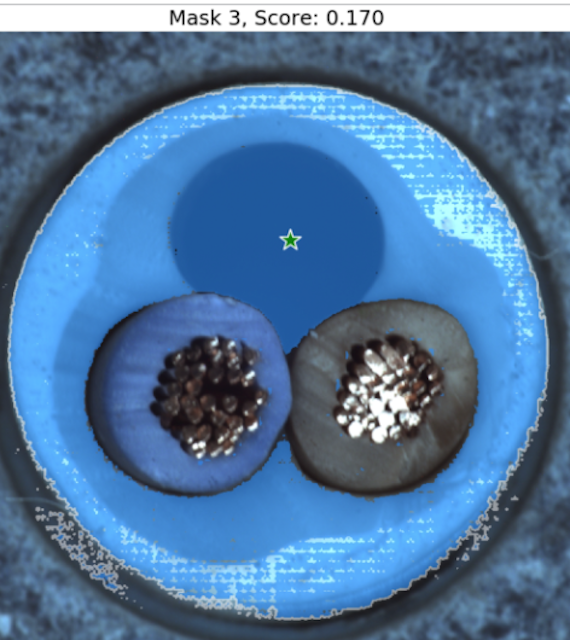
\includegraphics[width=0.19\linewidth]{figs/phase_1/missing_wire_5.png}

        % 情况4: failure case:不能分出结构,完全失败 (物体形变)
        % carpet
        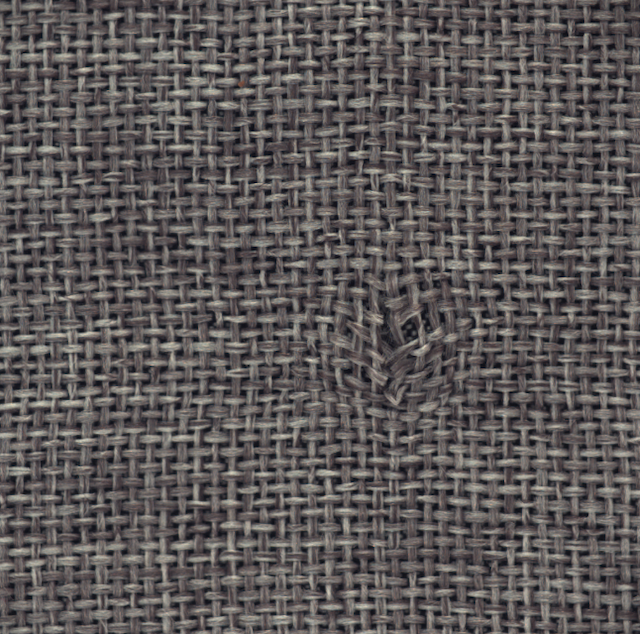
\includegraphics[width=0.19\linewidth]{figs/phase_1/carpet_1.png}
        
\includegraphics[width=0.19\linewidth]{figs/phase_1/carpet_2.png}
        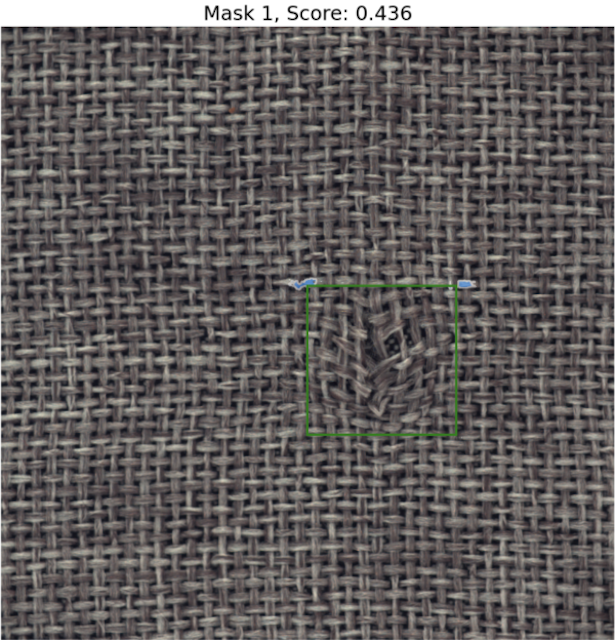
\includegraphics[width=0.19\linewidth]{figs/phase_1/carpet_3.png}
        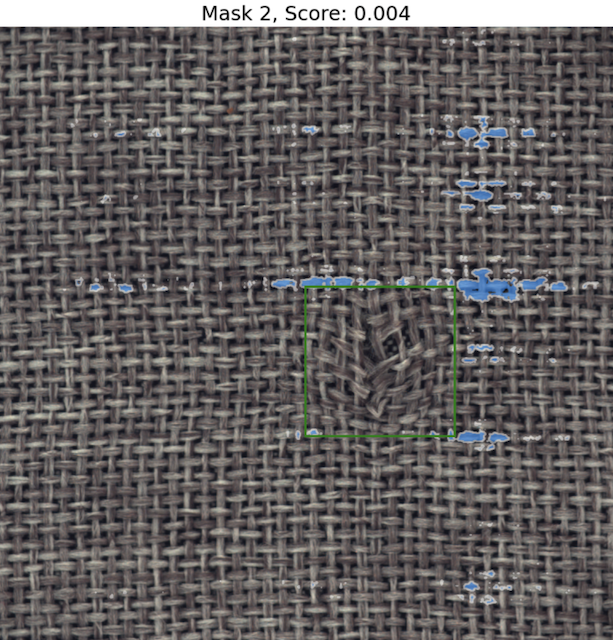
\includegraphics[width=0.19\linewidth]{figs/phase_1/carpet_4.png}
        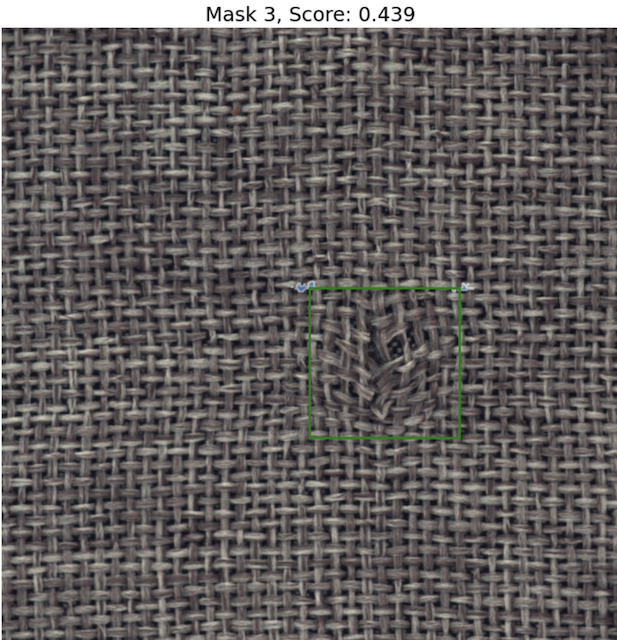
\includegraphics[width=0.19\linewidth]{figs/phase_1/carpet_5.png}
  
	\caption{Representative segmentation examples from SAM across four industrial anomaly cases. Each row shows (from left to right): the original input image, the ground truth segmentation mask, and three predicted masks generated by SAM. The scores shown above each predicted mask correspond to the model’s internal confidence estimate, computed as the predicted Intersection over Union (IoU) between the generated mask and its estimated ground truth. These scores reflect SAM’s own assessment of mask quality.}
        % \Description{}
	% \vspace{-.1in}
	\label{fig:sam_result}
\end{figure*}

\subsubsection{Finetuning Results: SFT-SAM vs. VisionSAM (RLHF)}
% 故事可以这么讲:RLHF(PPO)实现难度比较大、复杂 —> DPO, 但是说的时候要说另一套东西。

% \autoref{fig:sft_vs_rlhf}

% 1, SFT后的效果,能改善一些anomaly的情况。
% 2, 在SFT上进行DPO finetune会有微小提升,但是作用不大。在original SAM上进行DPO finetune会导致性能下降
% 需要说明为什么,原因分析
% 最后再解释一下 Figure 5的结果

% 对于table1: 经过SFT后,SFT-SAM对比原来的SAM性能在IoU指标和Dice指标分别提升了+~13.17%和 +~9.76%。经过RLHF后,VisionSAM对比SFT-SAM性能提升了+~0.43%和+~0.69%。结论:1,SFT后对性能有改善;2,但是VisionSAM相对来说效果不明显。这里可以refer to figure 5的右侧图片:右侧的图片是VisionSAM的分割结果,可以看到VisionSAM尝试去分割Wood这个物体上侧部分的刮痕,但是产生的是噪声点而不是将刮痕分割出来。

% 然后说明Figure 5: figure 5左边的图,SAM vs SFT-SAM;右边的图:SFT-SAM vs VisionSAM。

\autoref{tab:table1} summarizes the overall segmentation performance of the original SAM, the supervised fine-tuned variant (SFT-SAM), and the RLHF-enhanced model (VisionSAM). Compared to the original SAM, SFT-SAM achieves a substantial performance gain, with an IoU improvement of approximately +13.17\% and a Dice improvement of +9.76\%, demonstrating the effectiveness of domain-specific supervised finetuning. After further finetuning via RLHF, VisionSAM achieves a modest improvement over SFT-SAM, with an additional +0.43\% in IoU and +0.69\% in Dice. While this gain indicates that preference-based learning can further refine the model, the overall impact remains limited, suggesting that the benefits of RLHF are more subtle in the absence of large-scale or high-confidence feedback. This observation is further supported by the qualitative result shown in \autoref{fig:sft_vs_rlhf} (right). Although VisionSAM attempts to capture a subtle scratch on the upper part of a wooden surface, it fails to localize the anomaly effectively, producing scattered noise instead of a coherent segmentation mask.

% table1, 性能对比1: 三个模型
% Table generated by Excel2LaTeX from sheet 'Sheet1'
\begin{table}[htbp]
  \centering
  \caption{Overall segmentation performance of SAM, SFT-SAM, and \model.}
    \begin{tabular}{lccc}
    \toprule
          & \multicolumn{1}{l}{IoU} & Dice & Params Size \\
    \midrule
    SAM  & 0.5818  & 0.7049 & 357.1 M \\
    SFT-SAM & 0.6584 & 0.7737 & 357.1 M \\
    % RLHF-SAM & 0.5686 & 0.6931 & 375.1 M \\
    \model & 0.6612 \textsuperscript{↑} & 0.7790 \textsuperscript{↑} & 375.1 M \\
    \bottomrule
    \end{tabular}%
  \label{tab:table1}%
\end{table}%


% 对于table 2: 在SFT上进行DPO finetune会有微小提升,但是作用不大。在original SAM上进行DPO finetune会导致性能下降(downgrade), 这里需要分析可能的原因。 Another interesting thing to notice is that我们尝试用DPO直接finetune SAM, named RLHF-SAM,但是会导致性能下降(downgrade), IoU 下降2.27%, Dice下降1.67%

% direct RLHF on SAM degrades performance

% \autoref{tab:table2} Another interesting thing to notice is that

\autoref{tab:table2} presents the results of directly applying DPO-based preference finetuning on the original SAM model, resulting in RLHF-SAM. Interestingly, this approach leads to a performance drop: IoU decreases by 2.27\% and Dice by 1.67\% compared to the original SAM. This indicates that direct preference-based finetuning without prior supervised adaptation may be ineffective—or even harmful—in the anomaly segmentation setting. One plausible explanation is that the base SAM model lacks task-specific alignment prior to RLHF. Without supervised grounding on domain-relevant demonstrations, DPO optimization may attempt to align preference gradients on top of a representation that is not yet sensitive to the fine-grained anomaly features. Additionally, the human-labeled preferences may conflict with SAM’s original object-centric inductive biases, resulting in unstable or noisy updates when no intermediate supervised signal is provided. This result highlights the importance of using supervised finetuning as a warm start before applying RLHF techniques in dense prediction tasks like segmentation, where alignment targets are less well-defined than in language generation.

% table2, 性能对比2: 引出第二个结论: 如果将DPO应用在original SAM上的话,效果会不如应用在SFT上的效果。
% Table generated by Excel2LaTeX from sheet 'Sheet1'
\begin{table}[htbp]
  \centering
  \caption{Performance comparison between the original SAM and RLHF-SAM, where RLHF-SAM is obtained by directly applying DPO finetuning on the original SAM without prior supervised training.}
    \begin{tabular}{lccc}
    \toprule
          & \multicolumn{1}{l}{IoU} & Dice & Params Size \\
    \midrule
    SAM  & 0.5818  & 0.7049 & 357.1 M \\
    RLHF-SAM & 0.5686 \textsuperscript{↓} & 0.6931 \textsuperscript{↓} & 375.1 M \\
    \bottomrule
    \end{tabular}%
  \label{tab:table2}%
\end{table}%

\begin{figure*}[htbp]
  \centering
  \begin{subfigure}[t]{0.49\textwidth}
    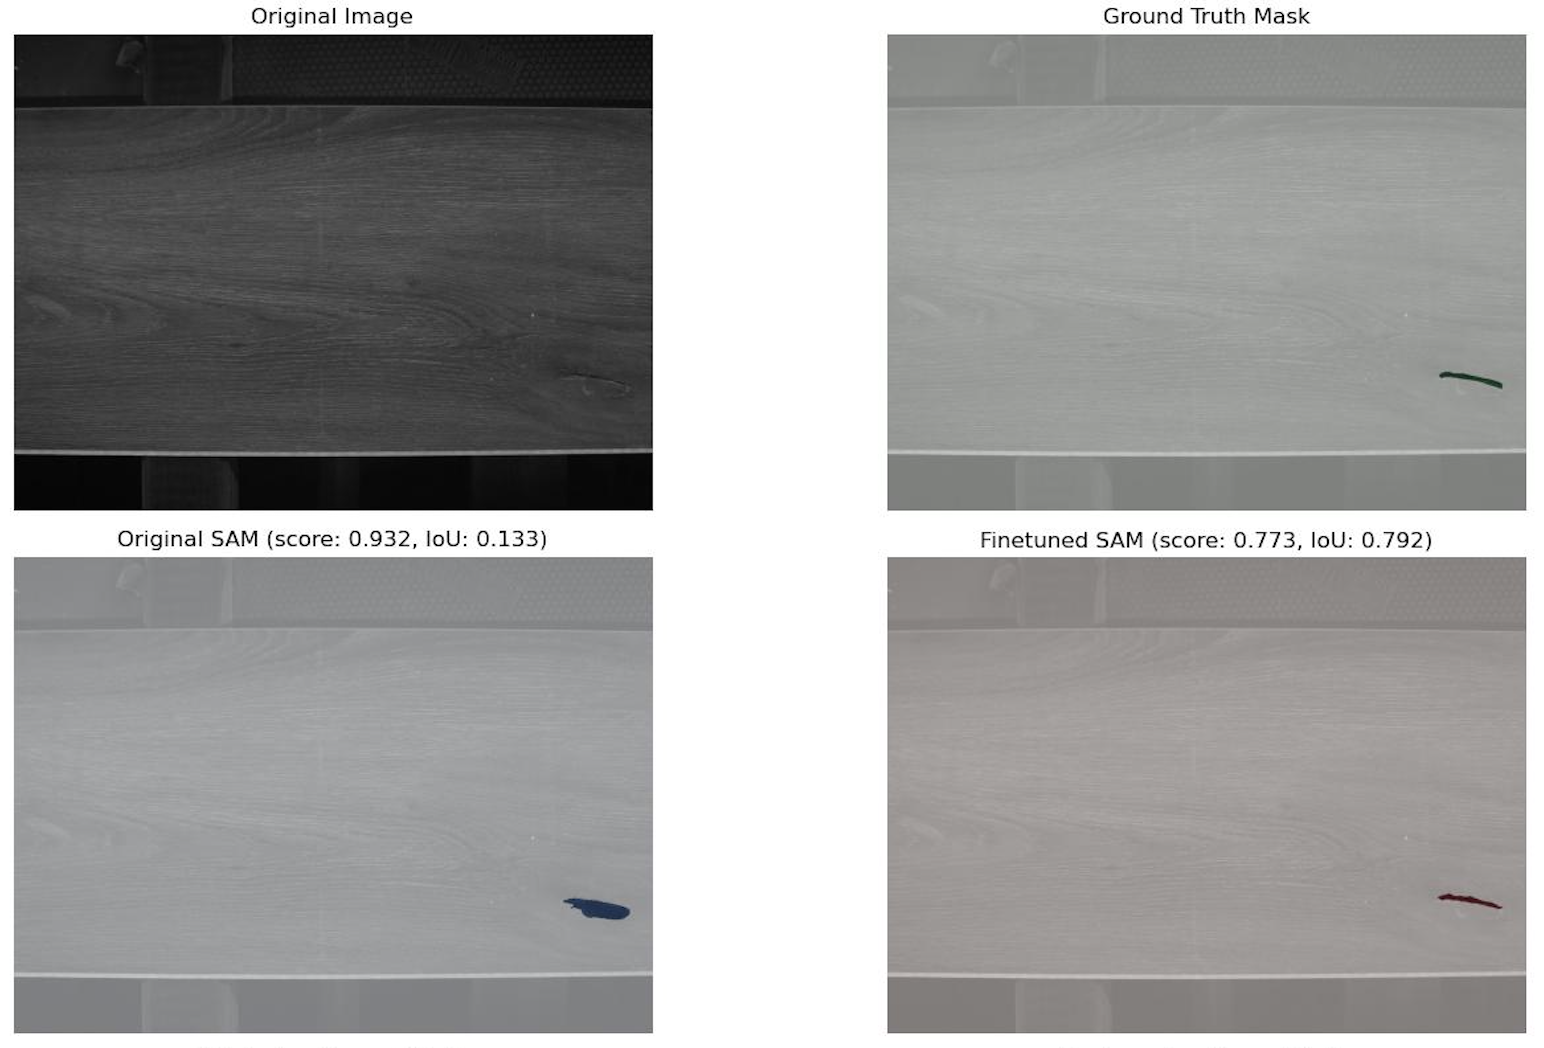
\includegraphics[width=\linewidth]{figs/wood_034.png}
    \caption{Comparison between the original SAM and SFT-SAM on an anomaly segmentation sample.}
  \end{subfigure}
  \hfill
  \begin{subfigure}[t]{0.49\textwidth}
    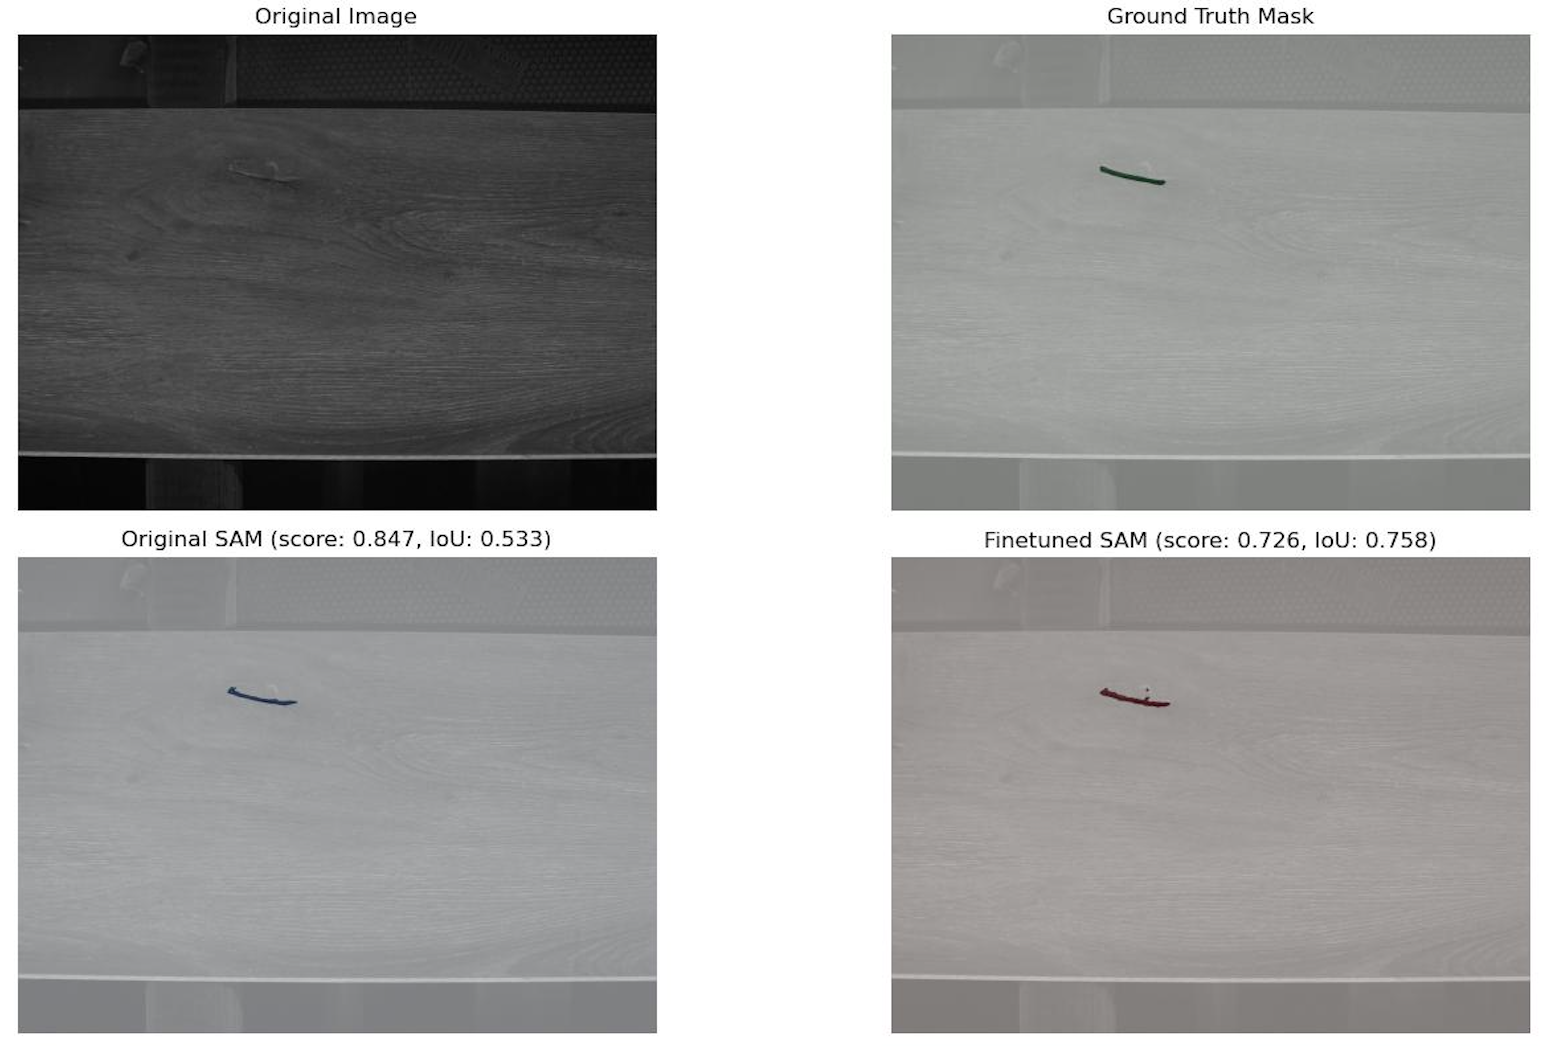
\includegraphics[width=\linewidth]{figs/wood_026_noise.png}
    \caption{Comparison between the SFT-SAM and \model on an anomaly segmentation sample.}
  \end{subfigure}
  \caption{Visualization of anomaly segmentation results across finetuning stages: (a) original SAM vs. SFT-SAM, and (b) SFT-SAM vs. \model.}
  \label{fig:sft_vs_rlhf}
\end{figure*}





% \textsuperscript{↓2.26\%}

% 放IoU和Dice的效果对比图。



\section{Discussion} 
% \subsection{Reproducibility, Data Use, and Ethical Considerations}
% Replicability+Datasets+Ethics 的内容不重要,只是为了拿分而已 (15 pts in total)
\textbf{Replicability.} To ensure replicability, we can provide all necessary code, training scripts, inference utilities, and model checkpoints, along with detailed documentation of hyperparameters and experimental settings if you request. Our pipeline is built on publicly available frameworks, and we fix random seeds to reduce variability across runs. 

\textbf{Datasets.} We reorganize a subset of the VISION anomaly segmentation dataset and introduce a small-scale preference-annotated comparison set constructed via human-in-the-loop labeling. Additionally, we use the publicly available MVTec-AD dataset for zero-shot evaluation of segmentation performance. The MVTec-AD dataset is released under the Creative Commons Attribution-NonCommercial-ShareAlike 4.0 International License (CC BY-NC-SA 4.0), which prohibits commercial use. Users who are unsure whether their application violates the non-commercial use clause are advised to contact the original dataset authors. We hope our annotations and benchmarking efforts encourage future research on incorporating human feedback into vision models in industrial settings.

\textbf{Ethics.} From an ethical standpoint, our work poses low direct societal risk, as it focuses exclusively on industrial anomaly segmentation without involving human subjects or sensitive personal data. However, we caution against the blind deployment of automated inspection systems, particularly in high-stakes industrial settings, and recommend incorporating human oversight in safety-critical applications. Notably, our preference annotations were collected by annotators from the same cultural and geographic background, which may introduce subtle bias in how anomalies are perceived and ranked. We encourage future research to explore more diverse human feedback and evaluate generalization across broader defect types and annotation perspectives.


% ------ Limitations --------
% 这里要强调模型的limitations而不是methods上的。这个部分可以详写。表明研究时遇到的困境,表明困境后,虽然暂时解决不了,但态度上要诚恳说明本论文的重要性以及可能的解决方法(解决方案要合理可行)。

% limitation 1: VisionSAM在RLHFfinetune后的表现以及性能提升不显著。
% limitation 2: While VisionSAM is balabla. It can miss fine structures, hallucinates small disconnected components at times, and does not produce boundaries as crisply as more computationally intensive methods balabala ...on some hard category.
% limitation 3: inference speed 的问题
\textbf{Limitations.} While our proposed VisionSAM demonstrates the feasibility of applying reinforcement learning from human feedback (RLHF) to industrial anomaly segmentation, several limitations remain. First, the overall performance gain from RLHF finetuning is modest, with only incremental improvements over the supervised finetuned baseline (SFT-SAM). This suggests that preference signals alone may not be sufficient to significantly shift the behavior of a model already aligned with the task via supervision. Second, although VisionSAM shows better alignment with human preferences in many cases, it occasionally struggles with capturing fine-grained structures, tends to hallucinate small disconnected components, and produces less precise boundaries compared to heavier segmentation models—particularly on challenging categories with low contrast or irregular defect patterns. Lastly, inference speed is another practical concern. While our method remains efficient in terms of model size, generating and comparing multiple masks for each prompt during inference incurs additional computational overhead.

% ------ Future Works --------
% 思考:如何将异常注入vision foundation model
% 根据模型的问题再针对性的提出几个可能的解决方案。
% 如果对于本实验的条件进行变更,提出一些新的问题和下一步的研究建议。
\textbf{Future Works.} Despite these limitations, our work highlights the potential of integrating RLHF into segmentation pipelines and contributes a reproducible framework for preference-based vision model optimization. Several possibilities remain for further improvement. One direction is to better inject the notion of “anomaly” into the model. Existing models like SAM are primarily object-centric and may overlook subtle defects; future work may consider pretraining on anomaly-centric datasets or designing prompts that more explicitly highlight abnormal regions. Additionally, our current preference annotations are based on binary comparisons (preferred vs. rejected), which provide limited feedback. Richer forms of supervision—such as ranked masks, region-level critiques, or confidence calibration from experts—could offer stronger learning signals. Finally, our comparison dataset is relatively small and annotated by individuals from similar cultural and professional backgrounds. Expanding both the dataset scale and annotator diversity across domains may lead to more generalizable and unbiased preference-aligned models.

% ------- Conclusion ------
% \textbf{Conclusion.}
% 重述全文的结论和成果,但不要重复Results已经说过的结果。着重点放在「讨论」,即对研究结果的意义进行分析,目的是清除阐述该研究解决了该领域中的具体问题。
% 这里可以略过

% -------- Acknowledgments -----
\textbf{Acknowledgments.} We would like to thank the reviewers for their valuable feedback throughout the project. We also appreciate the insightful discussions and suggestions from James Mooney, Risako Owan, Bin Hu, and Junhan Wu, as well as the thoughtful questions raised by peers during the poster session, which greatly inspired our thinking.

% Reference (2025/5/7: 还需要补充一些reference)
\bibliography{custom}
\nocite{*} % show all bibliography
% % \appendix

\section{Appendix}

% 可以放一个数据分布图在这里

\subsection{Q and A for Rubric: for TA's convenience}
Rubric QA is recorded in this \href{https://docs.google.com/spreadsheets/d/1W_pmCWLjmBhsGSjDms_AUPLtigZsEp_DR7B2RvcxRu8/edit?gid=1508992498#gid=1508992498}{google sheet} for TA's grading convenience.

\end{document}
